\chapter{Sistema de aproximación de la distancia}
\label{cha:Sistema de aproximación de la distancia}

\begin{FraseCelebre}
  \begin{Frase}
    Texto.
  \end{Frase}
  \begin{Fuente}
    Autor texto
  \end{Fuente}
\end{FraseCelebre}

\noindent
Obteniendo las detecciones 2D de los objetos dentro del \ac{FoV} de la cámara utilizada, se procede al estudio de los posibles métodos a utilizar para la aproximación de la distancia a cada uno de los objetos del entorno. Como técnicas a evaluar, en un principio se plantea: el uso de un método basado en una regresión utilizando las características más importantes que consigan predecir la distancia y la obtención directa la distancia mediante la proyección de la nube del puntos del \ac{LiDAR} sobre la cámara del vehículo; siendo ambas técnicas basadas en modelos clásicos de \ac{ML}.

El estudio y elección de los modelos de aproximación de la distancia se han realizada sobre cuadernos de trabajo Jupyter utilizando el lenguaje Python para simplificar el tratamiento de los datos, además de la necesidad de tratar con imágenes y nubes de puntos dentro de este apartado. Este trabajo se puede encontrar en en siguiente repositorio git alojado en GitHub, dentro de la carpeta 'Distance approximation': \url{https://github.com/Javier-DlaP/3D-detection-system-lidar-camera}.

\section{Análisis del dataset KITTI}
\label{sec:Análisis del dataset KITTI}

El primer paso dentro del proceso de creación de un modelo de \ac{ML} consiste en la comprensión de los datos con los que se está trabajo, por ello, en este primer apartado, se va a observar que datos de importancia aporta KITTI para la creación del modelo requerido.

Dentro del dataset de KITTI el ground-truth se encuentra guardado como un archivo de texto por cada uno de los 7.481 frames de datos guardados. En este ground-truth se observa la aparición de: coches, peatones, ciclistas, camiones y objetos desconocidos; pero ya que dentro del evaluador de KITTI solo se analizan: coches, peatones y ciclistas; se ha decidido estudiar únicamente estas clases \cite{kitti_evaluator_3d}. Con la elección de los datos a utilizar, se genera un script que unifica en un dataframe todos los archivos de ground-truth del dataset para poder analizarlos de forma más sencilla. Tras esto se consigue un dataframe con 34.856 objetos diferentes (únicamente de las clases: coche, peatón y cilista), en el que se recoge por cada objeto la información del: frame, identificador, tipo, visibilidad, rotación, bounding box 2D, dimensiones, centro tridimensional, etc. De forma adicional, se generan varias características extra que se espera que aporten información al estudio como: la distancia a cada objeto, la altura y anchura en píxeles de las bounding boxes 2D, y la completitud de las bounding boxes 2D en la componente vertical y horizontal debido a la aparición de objetos parcialmente visibles debido al \ac{FoV} de la cámara utilizada en este dataset. En cuanto al uso del dataframe para el ajuste y evaluación de los modelos a crear, se ha dividido dicho dataframe creado en dos diferentes, uno de entrenamiento y otro de evaluación atendiendo a la división dada por el dataset de KITTI.

\begin{figure}[H]
    \centering
    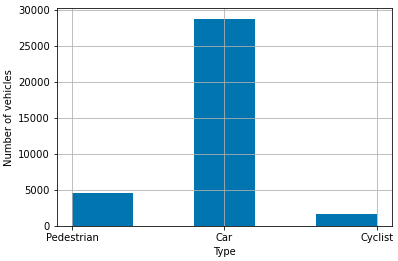
\includegraphics[width=0.4\textwidth]{Book/figures/6_approx_distancia/classes_kitti.png}
    \caption{Aparición de las clases en KITTI.}
    \label{fig:Aparición de las clases en KITTI.}
\end{figure}

Uno de los problemas más importantes a tener en cuenta dentro del dataset de KITTI es la pésima distribución de las clases con las que se trata. Como se observa en la Figura \ref{fig:Aparición de las clases en KITTI.}, en torno a un 80\% de objetos con los que se trabaja son coches por lo que es muy importante tener esto en cuenta, ya que no todas las clases tienen las misma características y puede influir negativamente en el ajuste de los modelos a diseñar. En cuanto a este hecho, la aplicación de técnicas de fine tuning presentadas en el Capítulo \ref{sec:Entrenamiento y evaluación de YOLOv5} para el entrenamiento del modelo de detección del objetos 2D consigue evitar parcialmente el sobreajuste que implica el uso de clases tan desbalanceadas.

\begin{figure}[H]
	\begin{minipage}{0.48\textwidth}
		\centering
		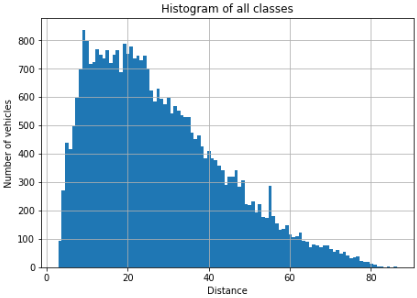
\includegraphics[width=0.97\linewidth]{Book/figures/6_approx_distancia/distance_kitti.png}
		\caption{Distribución de la distancia.}
		\label{fig:Distribución de la distancia.}
	\end{minipage}\hfill
	\begin{minipage}{0.45\textwidth}
		\centering
		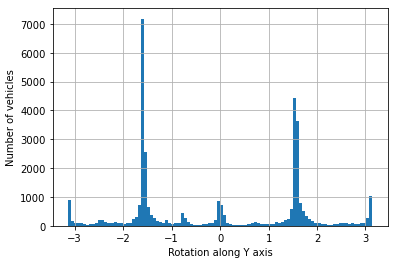
\includegraphics[width=1\linewidth]{Book/figures/6_approx_distancia/rotation_y_kitti.png}
		\caption{Distribución de la rotación.}
		\label{fig:Distribución de la rotación.}
	\end{minipage}
\end{figure}

De la misma que se ha  analizado los datos en relación al tipo de clase presente en el dataset, otras de las características más interesantes para su análisis son: la distribución de distancias a cada objeto del ground-truth y la rotación respecto del eje del propio vehículo del resto de objeto del entorno.

La Figura \ref{fig:Distribución de la distancia.} muestra la distribución de la distancia a los vehículos del ground-truth calculada como la distancia desde el origen del sistema de coordenadas de la cámara y el centro tridimensional de los objetos ($\sqrt{x^2+y^2+z^2}$). Esta distribución muestra como la mayoría de los objetos del ground-truth se encuentran entre los 10 y los 30 metros, además de encontrar objetos hasta una distancia de 80 metros, los cuales no se terminan evaluando debido a los diferentes niveles de dificultad que tiene KITTI (los cuales se presentarán más adelante) y que descartan el uso de estos objetos tan alejados. Estudiando la distancia por clases, se ha observado como los coches y ciclistas tienen su mayor presencia en torno a los 20 metros, mientras que los peatones tienen una mayor aparición a los 10 metros. En el caso de la detección 3D de los objetos se pretende conseguir unas detecciones relativamente buenas hasta los 50 metros, ya que a partir de esa distancia, se trabaja con muy pocos píxeles en la cámara y apenas puntos del \ac{LiDAR} lo que resulta en una tarea extremadamente compleja.

En cuanto a la rotación de los objetos del entorno respecto del vehículo propio, en la Figura \ref{fig:Distribución de la rotación.} se puede ver como los valores cercanos a $\pi/2$ y $-\pi/2$ son aquellos más prevalecientes en el dataset. Esto es debido a que este campo utiliza un sistema de rotación medido radianes donde el 0 apunta hacia la derecha del propio vehículo en \ac{BEV}. Por lo que se puede asumir directamente que lo más probable en cuanto a la orientación de todos los objetos de ground-truth es que se encuentren en la misma dirección pero puede ser el sentido puede ser el mismo o el opuesto, esto es muy probablemente debido a que la mayoría de los objetos del entorno a detectar se encuentran en los carriles, por lo que excepto en intersecciones esto va a ser correcto.

\begin{figure}[H]
    \centering
    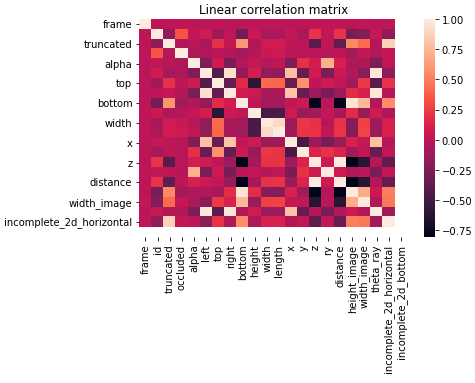
\includegraphics[width=0.6\textwidth]{Book/figures/6_approx_distancia/corr_matrix_kitti.png}
    \caption{Matriz de correlación de las características analizadas.}
    \label{fig:Matriz de correlación de las características analizadas.}
\end{figure}

Dentro de este mismo análisis se estudia de manera muy superficial las características del dataset que tienen una mayor relación con la distancia ya que es necesario obtener con que característica se puede obtener la distancia, tal y como se tratará se realizar en el siguiente capítulo. Para ello se construye una matriz de correlación mediante el uso del coeficiente de correlación de Pearson: $\rho_{X,Y} = \sigma_{X,Y}/(\sigma_X \sigma_Y)$. La Figura \ref{fig:Matriz de correlación de las características analizadas.} muestra dicha matriz de correlación en la que se observa como son: la recta horizontal inferior de la bounding box 2D, el eje Z del centro tridimensional, la altura de la bounding box 2D y la anchura de la bounding box 2D; aquellos parámetros que tienen un índice de correlación mayor con la distancia.

Habiendo obtenido las características más relevantes para la obtención de la distancia a los objetos, se visualiza en un gráfico de dispersión con la relación entre estos y la distancia, para obtener la característica a utilizar en la predicción de la distancia. La Figura \ref{fig:Gráficos de dispersión entre la distancia y las características con más correlación.} muestra todos los gráficos de dispersión, teniendo en el eje de ordenadas la distancia a los objetos y en el eje de abscisas las características estudiadas. En este gráfico se observa como a partir del eje Z del centro tridimensional se puede obtener directamente la distancia, de forma adicional, a partir de la recta horizontal inferior de la bounding box 2D y la altura de la bounding box 2D se puede obtener también la distancia pero con algo más de error, por último, con la la anchura de la bounding box 2D no se puede obtener la distancia de forma sencilla sin asumir un error muy grande.

\begin{figure}[H]
    \centering
    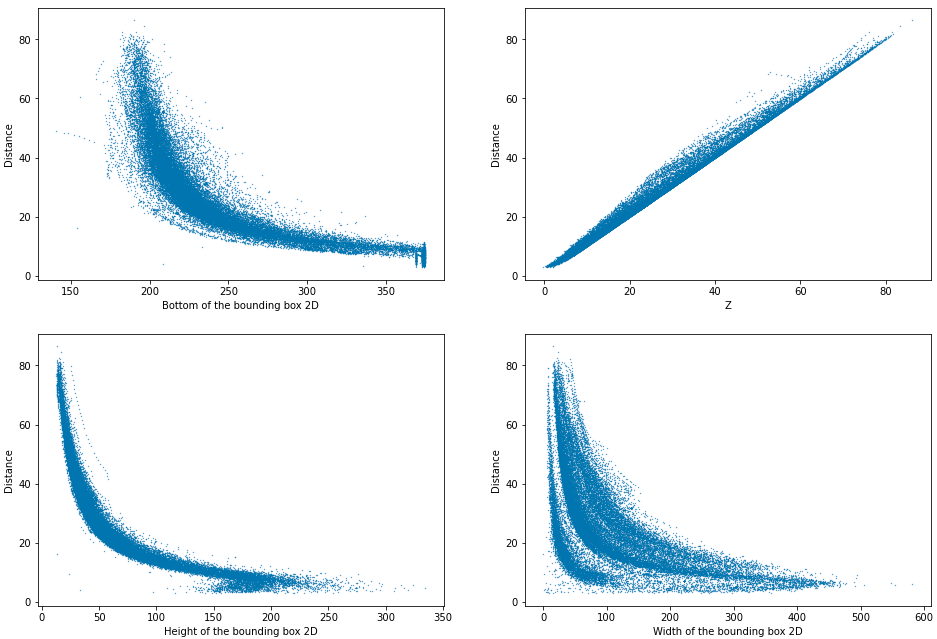
\includegraphics[width=0.9\textwidth]{Book/figures/6_approx_distancia/metrics_to_get_distance_kitti.png}
    \caption{Gráficos de dispersión entre la distancia y las características con más correlación.}
    \label{fig:Gráficos de dispersión entre la distancia y las características con más correlación.}
\end{figure}

Debido a que el eje Z del centro tridimensional de los objetos no se conoce de antemano, se decide utilizar para obtener la distancia a los objetos, la altura de la bounding box 2D. Esto es así, ya que de forma comparativa con la recta horizontal inferior de la bounding box 2D, se tiene una menor dispersión, además de estar asumiendo con este parámetro que el vehículo se encuentra siempre en una carretera sin pendientes, ya que el dataset de KITTI no contiene ninguna situación con esta característica.

\section{Modelo basado en la altura del objeto 2D}
\label{sec:Modelo basado en la altura del objeto 2D}

Habiendo elegido la característica que permite de mejor manera la obtención de la distancia, se trata de obtener una función que ajuste la distancia tras la obtención de la bounding box 2D de cada objeto. Este ajuste de la función no se realiza sobre la salida del modelo \ac{YOLO}v5, sino que parte del ground-truth de KITTI para su ajuste con los datos de entrenamiento, y se comprueba la efectividad de dicho ajuste sobre los datos de validación.

La métrica definida para la evaluación de todos los modelos de aproximación de la distancia es el \ac{MSE}, el cual se define por la siguiente función: $\textit{MSE} = \frac{1}{n} \sum_{i=1}^{n} (Y_i - \hat{Y}_i)^2$. Esta métrica es elegida ya que elimina los errores positivos y negativos, además de castigar de forma cuadrática los errores más grandes, lo cual permitirá discernir de mejor manera el modelo que más se ajusta.

En cuanto al modelo de ajuste, se decide optar por un sencillo modelo de regresión (no lineal) ya que permite su creación de forma sencilla además de permitir una ejecución de forma inmediata sin añadir carga de trabajo a todo el pipeline de detección 3D. Para realizar el ajuste de la función a utilizar que tenga de entrada la altura de la bounding box 2D y como salida la distancia al objeto, se utiliza la librería Scikit-learn. Mediante el uso de dicha librería en Python, se definen múltiples funciones polinómicas y logarítmicas para que mediante un ajuste por mínimos cuadrados se obtengan los valores que compongan las diferentes funciones.

En la Figura \ref{fig:Ajuste de diversas funciones para la obtención de la distancia.} se observan 6 de las funciones que se han probado para ajustar la obtención de la distancia. En esta imagen se observa como las funciones polinómicas no son capaces de ajustarse de forma correcta a las características de la curva definida por la relación entre las características analizadas. Por otra parte, las funciones funciones logarítmicas utilizadas son aquellas que mejor se ajustan, siendo la siguiente función aquella que mejor se ajusta: $y = a \log{x}^b + c; a = 668,12; b = -2; c = -17,39$.

\begin{figure}[H]
    \centering
    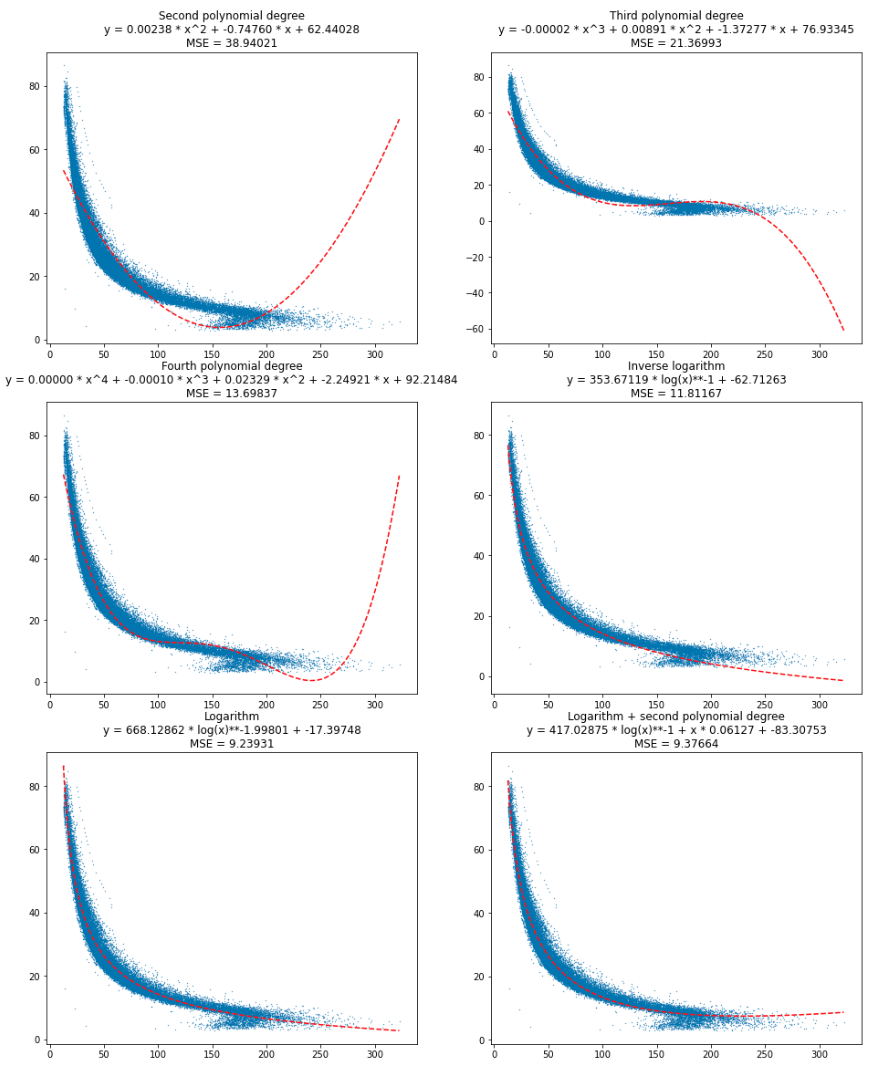
\includegraphics[width=0.7\textwidth]{Book/figures/6_approx_distancia/distance_regression_1_kitti1.png}
    \caption{Ajuste de diversas funciones para la obtención de la distancia.}
    \label{fig:Ajuste de diversas funciones para la obtención de la distancia.}
\end{figure}

Habiendo observado en el capítulo anterior que cada una de las clases de objetos utilizados tiene unas dimensiones diferentes, se plantea la creación de una función por cada una de las tres clases a detectar. Para ello se utilizará la función logarítmica previamente obtenida que se ajusta de mejor manera a los datos.

Tras la obtención de las parámetros de esta función logarítmica se obtienen las diferentes curvas que ajustan la relación entre la distancia y altura de la bounding box 2D para cada una de las clases. Esto se realiza de esta manera debido a que la altura media de cada una de las clases es diferente, por lo que el ajuste al realizarse de forma individual por cada clase de puede mejorar la precisión de las predicciones de la distancia a cada objeto. En la Figura \ref{fig:Ajuste de una función logarítmica por cada clase.} se observa como en las clases peatón y ciclista la métrica de \ac{MSE} se reduce, mientras que en la clase coche se aumenta. Esto es debido a que como se vio previamente, el 80\% de los objetos de los objetos son coches, por lo que se les puede encontrar en muchas más situaciones complejas.

\begin{figure}[H]
    \centering
    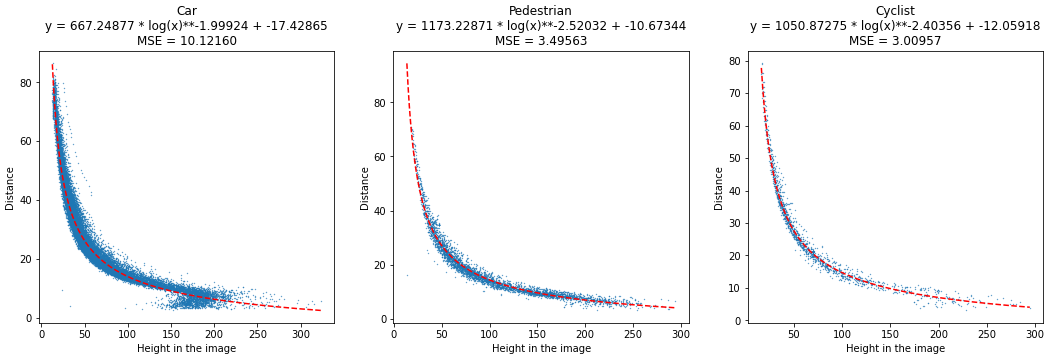
\includegraphics[width=1\textwidth]{Book/figures/6_approx_distancia/regression_classes_kitti1.png}
    \caption{Ajuste de una función logarítmica por cada clase.}
    \label{fig:Ajuste de una función logarítmica por cada clase.}
\end{figure}

Analizando el resto de características con las que se puede trabajar para obtener una aproximación de la distancia más precisa, se encuentra que la completitud horizontal de las bounding boxes 2D de los objetos, definida como aquellas bounding boxes que se encuentran en el límite izquierdo o derecho de la imagen, pueden aportar información al modelo, ya que aquellas bounding boxes que cumplen esta propiedad, no se conoce de forma correcta la altura de su bounding box 2D al no encontrarse el objeto al completo dentro del \ac{FoV} de la cámara. Se ha observado de forma adicional, como el análisis únicamente de la componente horizontal de la bounding box 2D aporta más información que el uso de la componente vertical o la combinación de ambas.

En la Figura \ref{fig:Resaltado de las bounding box 2D no completas horizontalmente.} se puede ver de forma resaltada en naranja aquellos objetos que cumplen con el filtro de bounding boxes 2D incompletas horizontalmente. En dichos puntos naranjas se observa una distribución diferente a la encontrada de forma general en el resto del dataset, por lo que se decide incorporar este parámetro al modelo a utilizar. 

\begin{figure}[H]
    \centering
    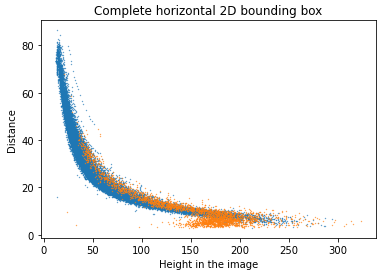
\includegraphics[width=0.5\textwidth]{Book/figures/6_approx_distancia/bb_complete_kitti1.png}
    \caption{Resaltado de las bounding box 2D no completas horizontalmente.}
    \label{fig:Resaltado de las bounding box 2D no completas horizontalmente.}
\end{figure}

Habiendo definido el uso de una nueva característica es necesario definir con que técnica tratarla, en este caso, al observarse en la figura anterior una nueva curva con los datos filtrados según la nueva característica a utilizar se decide ajustar de forma separada dos curvas logarítmicas como se ha hecho previamente. Durante el análisis de esta característica se ha observado que en las clases 'peatón' y 'ciclista' hay muy pocos casos en los que las bounding boxes 2D no se encuentren completas, debido a esto, para evitar un caso de sobreajuste se decide utilizar la clase 'coche' como la única por la que filtrar y ajustar una función en relación a la completitud de la bounding box 2D.

En la Figura \ref{fig:Ajuste de la distancia a los coches en función de la completitud de la bounding box 2D.} se muestra el ajuste de las dos curvas en función de la nueva característica a introducir en el modelo sobre la clase 'coche', de esta manera se consigue que las vehículos que cumplen esta característica tengan una distancia aproximada más precisa.

\begin{figure}[H]
	\begin{minipage}{0.45\textwidth}
		\centering
		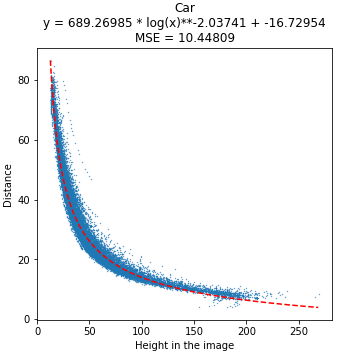
\includegraphics[width=0.87\linewidth]{Book/figures/6_approx_distancia/car_bb_complete_kitti1.png}
	\end{minipage}\hfill
	\begin{minipage}{0.45\textwidth}
		\centering
		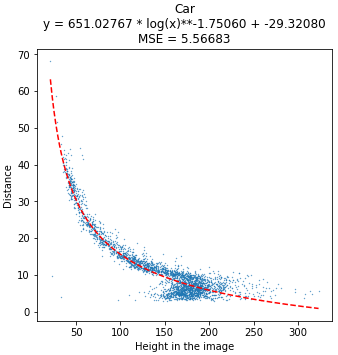
\includegraphics[width=0.9\linewidth]{Book/figures/6_approx_distancia/car_bb_incomplete_kitti1.png}
	\end{minipage}
	\caption{Ajuste de la distancia a los coches en función de la completitud de la bounding box 2D.}
	\label{fig:Ajuste de la distancia a los coches en función de la completitud de la bounding box 2D.}
\end{figure}

Como forma de estudiar los resultados obtenidos del sistema de aproximación de la distancia, se decide utilizar un método de evaluación común entre todos los modelos que sean diseñados, para ello se va a basar en el método de evaluación de KITTI y la métrica definida hasta ahora como es el \ac{MSE}.

Dentro de la evaluación de KITTI se define el concepto de dificultad entre los diferentes objetos a detectar, para los cuales se usa la altura de los objetos sobre la imagen, la oclusión (valor en función de la visibilidad del objeto que puede variar de 0 a 3) y el porcentaje de truncamiento de los objetos sobre el \ac{FoV} de la cámara. las diferentes dificultades con las que se trabaja son:
\begin{itemize}
    \item 'Fácil': son aquellos objetos con una altura en la imagen mayor de 40 píxeles, un valor de oclusión de 0 y un truncamiento máximo del 15\%.
    \item 'Moderado': son aquellos objetos con una altura en la imagen mayor de 25 píxeles, un valor de oclusión máximo de 1 y un truncamiento máximo del 30\%.
    \item Difícil: son aquellos objetos con una altura en la imagen mayor de 25 píxeles, un valor de oclusión máximo de 2 y un truncamiento máximo del 30\%.
\end{itemize}
El resto de los objetos que no se incluyen en ninguna de las diferentes categorías no se estudian, aunque más adelante se verá un caso en el que aquellos objetos sin dificultad han sido de relevancia.

Tras la definición del método de evaluación que se compone de las dificultades, la métrica (\ac{MSE}) y el estudio a nivel de clase, se calculan las métricas obtenidas en este primer método de aproximación de la distancia basado en la altura de las bounding boxes 2D.

\begin{table}[H]
\centering
\begin{tabular}{|c|c|c|c|}
\hline
\textbf{Benchmark (MSE)} & \textbf{Fácil} & \textbf{Moderado} & \textbf{Difícil} \\ \hline \hline
Coche (distancia)        & 8,724          & 9,115             & 9,127            \\ \hline
Peatón (distancia)       & 4,643          & 5,902             & 5,645            \\ \hline
Ciclista (distancia)     & 3,822          & 4,444             & 4,469            \\ \hline
\end{tabular}
\caption{Evaluación sobre KITTI del modelo de aproximación de distancia basado en regresión.}
\label{tab:Evaluación sobre KITTI del modelo de aproximación de distancia basado en regresión.}
\end{table}

La Tabla \ref{tab:Evaluación sobre KITTI del modelo de aproximación de distancia basado en regresión.} muestra unos resultados bastante buenos de este modelo de aproximación de distancia, el cual solo requiere de una imagen de las bounding boxes 2D que pueden ser obtenidas por un modelo como YOLOv5. Tras este primer modelo se estudiaran otros que traten de mejorar estos primeros resultados que son claramente bastante buenos pero mejorables.

\section{Modelo basado en la proyección de la nube de puntos}
\label{sec:Modelo basado en la proyección de la nube de puntos}

Habiendo obtenido un modelo de aproximación de la distancia basado únicamente en la cámara del vehículo, se ha decido utilizar también en un modelo diferente la nube de puntos proporcionada por el \ac{LiDAR}. Mientras que la cámara no tiene ningún método directo con el que calcular la distancia a los objetos, con el \ac{LiDAR} se puede calcular la distancia a cualquier punto de la nube de puntos obtenida por dicho sensor de forma precisa.

Partiendo del uso de bounding boxes 2D que pueden ser obtenidas por el modelo YOLOv5 presentado en la Sección \ref{sec:Entrenamiento y evaluación de YOLOv5}, se decide trabajar de forma conjunta con dichas detecciones 2D junto con el \ac{LiDAR} para analizar los puntos que se encuentran dentro de las bounding boxes. Mientras que esto parece una tarea sencilla es necesario estudiar las transformaciones de mundo a cámara de una lente como se observa en la Figura \ref{fig:Transformaciones mundo a cámara.} para poder pasar del sistema de coordenadas del LiDAR a la cámara.

\begin{figure}[H]
    \centering
    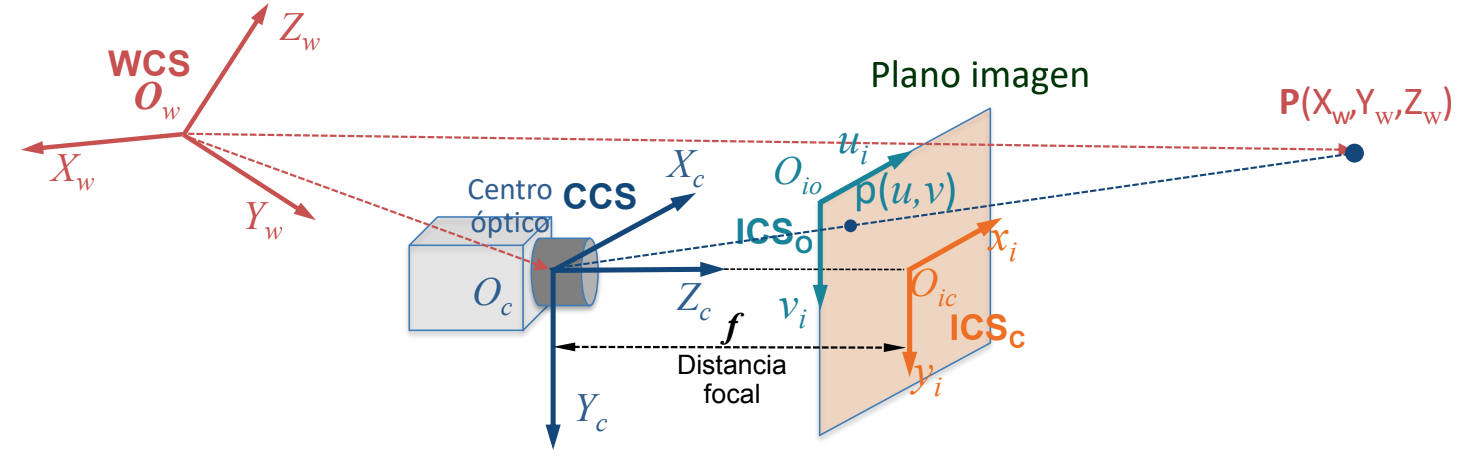
\includegraphics[width=0.7\textwidth]{Book/figures/6_approx_distancia/funcionamiento_camara.png}
    \caption{Transformaciones mundo a cámara.}
    \label{fig:Transformaciones mundo a cámara.}
\end{figure}

Tras el estudio de las transformaciones necesarias para obtener la nube de puntos sobre las imágenes obtenidas por la cámara se estudiaran los puntos para tratar de obtener un modelo que mejore al modelo anterior basado únicamente en la cámara. Para ello se plantea utilizar la mediana de la distancia de los puntos dentro de cada objeto y posteriormente se aplicará un pequeño modelo que obtenga la distancia al centro de cada objeto.

\subsection{Sistema de proyección de la nube de puntos a la cámara}
\label{sec:Sistema de proyección de la nube de puntos a la cámara}

Las nubes de puntos dadas en el dataset de KITTI siguen un formato típico en el cual a partir de un archivo binario se guarda la información de cada punto definida por los parámetros: 'x', 'y', 'z' y 'intensidad'; los cuales tienen un formato de números decimales de 32 bits. Dentro de las transformaciones geométricas a realizar solo es necesario utilizar las coordenadas tridimensionales de cada punto para realizar la traslación, rotación y cambio en el sistema de coordenadas de la nube de puntos. Para la comprensión de las operaciones realizadas en esta transformación es necesario comprender primero el funcionamiento de las proyecciones mundo a cámara las cuales son utilizadas en dicha proyección.

Como primer paso dentro de este proceso de la proyección de la nube de puntos a la cámara, es necesario el sistema de coordenadas a utilizar. En este caso se ha definido un sistema de coordenadas homogéneas para simplificar ciertos pasos más adelante, por lo que es necesario transformar el sistema de coordenadas cartesiano a este sistema de la manera definida por las siguientes fórmulas.

\begin{center}
$(x, y, z) \rightarrow (x', y', z', w)$\\[10pt]
$(x, y, z) = (x'/w, y'/w, z'/w)$
\end{center}

Tras la transformación al sistema de coordenadas homogéneo, se trata de cambiar el sistema de coordenadas actual al dado por la cámara con la que se trabaja, para ello es necesario realizar una traslación al sistema de coordenadas de la cámara y tras esto una rotación de los ejes para que concuerden con el sistema de coordenadas de la cámara. Al trabajar con las coordenadas homogéneas, la traslación del eje de coordenadas no es más que una multiplicación de matrices como se puede observa en la siguiente fórmula.

\begin{center}
$
\begin{bmatrix} wX_c \\ wY_c \\ wZ_c \\ w \end{bmatrix}
=
\begin{bmatrix}
1 & 0 & 0 & T_X \\
0 & 1 & 0 & T_Y \\
0 & 0 & 1 & T_Z \\
0 & 0 & 0 & 1 \\
\end{bmatrix}
\begin{bmatrix} X_w \\ Y_w \\ Z_w \\ 1 \end{bmatrix}
$
\end{center}

En cuanto a la rotación del sistema de coordenadas, es necesario entender que la rotación se realiza en los tres diferentes ejes, por lo que hay que utilizar una matriz de rotación por cada uno de los ejes, lo cual es una multiplicación de cuatro matrices.

\begin{center}
$R = R_X(\alpha) R_Y(\beta) R_Z(\gamma)$
\end{center}

\begin{center}
$
\begin{bmatrix} wX_c \\ wY_c \\ wZ_c \\ w \end{bmatrix}
=
\begin{bmatrix}
1 & 0 & 0 & 0 \\
0 & \cos \alpha & -\sin \alpha & 0 \\
0 & \sin \alpha & \cos \alpha & 0 \\
0 & 0 & 0 & 1 \\
\end{bmatrix}
\begin{bmatrix}
\cos \beta & 0 & \sin \beta & 0 \\
0 & 1 & 0 & 0 \\
- \sin \beta & 0 & \cos \beta & 0 \\
0 & 0 & 0 & 1 \\
\end{bmatrix}
\begin{bmatrix}
\cos \gamma & - \sin \gamma & 0 & 0 \\
\sin \gamma & \cos \gamma & 0 & 0 \\
0 & 0 & 1 & 0 \\
0 & 0 & 0 & 1 \\
\end{bmatrix}
\begin{bmatrix} X_w \\ Y_w \\ Z_w \\ 1 \end{bmatrix}
$
\end{center}

Otra opción es multiplicar desde un principio la matriz de traslación y las tres matrices de rotación que son fijas si no se mueve ninguno de los dos sistemas de coordenadas con los que se trabaja, y trabajar con una única matriz para reducir la complejidad de la fórmula además de reducir el numero de operación a realizar por un ordenador. Esta matriz es denominada la matriz de parámetros extrínsecos.

\begin{center}
$
\begin{bmatrix} wX_c \\ wY_c \\ wZ_c \\ w \end{bmatrix}
=
\begin{bmatrix}
\cos \gamma \cos \beta & - \sin \gamma \cos \beta & \sin \beta & T_X \\
\cos \gamma \sin \alpha \sin \beta + \sin \gamma \cos \alpha & \cos \gamma \cos \alpha - \sin \gamma \sin \alpha \sin \beta & - \sin \alpha \cos \beta & T_Y \\
\sin \gamma \sin \alpha - \cos \gamma \cos \alpha \sin \beta & \sin \gamma \cos \alpha \sin \beta + \cos \gamma \sin \alpha & \cos \alpha \cos \beta & T_Z \\
0 & 0 & 0 & 1 \\
\end{bmatrix}
\begin{bmatrix} X_w \\ Y_w \\ Z_w \\ 1 \end{bmatrix}
$
$
M_{ext}
=
\begin{bmatrix}
r_{11} & r_{12} & r_{13} & t_X \\
r_{21} & r_{22} & r_{23} & t_Y \\
r_{31} & r_{32} & r_{33} & t_Z \\
\end{bmatrix}
$
\end{center}

Tras este cambio del sistema de coordenadas al mismo con el que trabaja la cámara, es necesario pasar a nivel de píxel para comprender como cada punto del entorno tridimensional pasa a encontrarse dentro de las imágenes producidas por una cámara. Dentro de este proceso, es necesario comprender los parámetros intrínsecos que afectan en el paso del mundo real tridimensional al mundo bidimensional de las imágenes.

El primer parámetro a tener en cuenta es la distancia focal ($f$), la cual es la distancia entre el centro óptico de la lente y el foco de la cámara. Este parámetro es utilizado para pasar al sistema de coordenadas bidimensionales de la cámara pero en el sistema métrico.

\begin{center}
$
\begin{bmatrix} wx \\ wy \\ w \end{bmatrix}
=
\begin{bmatrix}
f & 0 & 0 & 0 \\
0 & f & 0 & 0 \\
0 & 0 & 1 & 0 \\
\end{bmatrix}
\begin{bmatrix} X_c \\ Y_c \\ Z_c \\ 1 \end{bmatrix}
$
\end{center}

Para obtener los puntos proyectados en los píxeles de las imágenes, se pasa al sistema de coordenadas pixélicas, definido por el tamaño en píxeles ($dx$, $dy$) y el desplazamiento al origen de las imágenes ($u_0$, $v_0$).

\begin{center}
$
\begin{bmatrix} wu \\ wv \\ w \end{bmatrix}
=
\begin{bmatrix}
1/dx & 0 & u_0 \\
0 & 1/dy & v_0 \\
0 & 0 & 1 \\
\end{bmatrix}
\begin{bmatrix} wx \\ wy \\ w \end{bmatrix}
$
\end{center}

De la misma manera que se construye la matriz de parámetros extrínsecos, se multiplican las dos últimas matrices relacionadas con los parámetros internos de la cámara, para construir una matriz de parámetros intrínsecos y simplificar el tratamiento de una cámara dada, ya que estos parámetros son fijos a una cámara concreta y no se modifican.

\begin{center}
$
M_{int}
=
\begin{bmatrix}
1/dx & 0 & u_0 \\
0 & 1/dy & v_0 \\
0 & 0 & 1 \\
\end{bmatrix}
\begin{bmatrix}
f & 0 & 0 \\
0 & f & 0 \\
0 & 0 & 1 \\
\end{bmatrix}
=
\begin{bmatrix}
f/dx & 0 & u_0 \\
0 & f/dy & v_0 \\
0 & 0 & 1 \\
\end{bmatrix}
$
\end{center}

De forma sencilla, se puede obtener la transformación de puntos tridimensionales del entorno a la cámara a partir de las matrices de parámetros extrínsecos e intrínsecos con unas simples multiplicaciones.

\begin{center}
$
\begin{bmatrix} wu \\ wv \\ w \end{bmatrix}
=
M_{int} M_{ext}
\begin{bmatrix} X_w \\ Y_w \\ Z_w \\ 1 \end{bmatrix}
$
\end{center}

Hasta ahora se ha explicado de forma teórica como funcionan las transformaciones necesarias para trabajar con cámara y comprender su tratamiento, pero en este apartado se explicará su uso práctico a partir de las matrices de calibración dadas en el dataset de KITTI y que han tenido que ser utilizadas para realizar todas las transformaciones geométricas necesarias en este apartado para la proyección de la nube de puntos además de su uso en la creación de 'troncos geométricos' como se verá en el Capítulo \ref{cha:Obtención de la región de interés}.

En este caso de uso concreto que se quiere obtener, es necesario trabajar con tres matrices diferentes con las que se logrará pasar del sistema de coordenadas de las nubes de puntos del \ac{LiDAR} a los píxeles de las imágenes dadas por el dataset de KITTI. Estas tres matrices son (según los nombres de dados por KITTI) las siguientes:

\begin{itemize}
    \item $P2$: Esta matriz se compone de la matriz intrínseca de la cámara 2, la cual es la cámara de la cual se van a utilizar las imágenes al ser aquella según se dan las detección 2D además de estar en color y no en escala de grises, además de la traslación respecto de la cámara 0 del vehículo utilizado para la creación de dataset.
    \item $R0\_rect$: Las lentes de la una cámara es muy difícil que sean perfectas, por lo que se suele aplicar una matriz de rectificación que tiene como función eliminar las imperfecciones en las imágenes como pueden ser las distorsiones de barril y de cojín. Esta matriz trata de solucionar estos problemas de las imágenes obtenidas por el sensor de la misma manera que se realiza con cual otro tipo de cámara (a menos que se trabaja con una lente con un error mínimo).
    \begin{center}
    $
    \textit{R0\_rect} = R_{Xr}(\alpha_r) R_{Yr}(\beta_r) R_{Zr}(\gamma_r) 
    \begin{bmatrix} 1&0&0&T_{Xr} \\ 0&1&0&T_{Yr} \\ 0&0&1&T_{Zr} \\ 0&0&0&1 \end{bmatrix}
    $
    \end{center}
    \item $Tr\_velo\_to\_cam$: Esta matriz se compone de la matriz de traslación del sistema de coordenadas del \ac{LiDAR} al sistema de coordenadas de la cámara 0 y de su correspondiente matriz de rotación.
    \begin{center}
    $
    \textit{Tr\_velo\_to\_cam} = R_{X\textit{v2c}}(\alpha_\textit{v2c}) R_{Yr}(\beta_\textit{v2c}) R_{Z\textit{v2c}}(\gamma_\textit{v2c}) 
    \begin{bmatrix} 1&0&0&T_{X\textit{v2c}} \\ 0&1&0&T_{Y\textit{v2c}} \\ 0&0&1&T_{Z\textit{v2c}} \\ 0&0&0&1 \end{bmatrix}
    $
    \end{center}
\end{itemize}

La conversión de la nube de puntos a las imágenes del dataset es muy sencilla si se conoce el funcionamiento de todas estas matriz, ya que simplemente es necesario multiplicar la nube de puntos completa por otras tres matrices diferentes como son: $P2$, $R0\_rect$ y $Tr\_velo\_to\_cam$.

\begin{center}
$
\textit{cam} = \textit{P2} * \textit{R0\_rect} * \textit{Tr\_velo\_to\_cam} * \textit{pcl}
$
\end{center}

\subsection{Aproximación de la distancia a partir de la nube de puntos}
\label{sec:Aproximación de la distancia a partir de la nube de puntos}

Partiendo del hecho que se conoce la manera de proyectar las nubes de puntos sobre las imágenes dadas, se abre una oportunidad para estudiar la distancia a los objetos a partir de dicha nube de puntos y las detecciones 2D que se pueden obtener de los objetos del entorno. La Figura \ref{fig:Proyección de la nube de puntos sobre la cámara.} muestra la manera en la que se proyecta la nube de puntos sobre la imagen que se da de entrada visualizando con colores la distancia del objeto con el colisiona cada láser del \ac{LiDAR} representado por un punto en la imagen.

\begin{figure}[H]
    \centering
    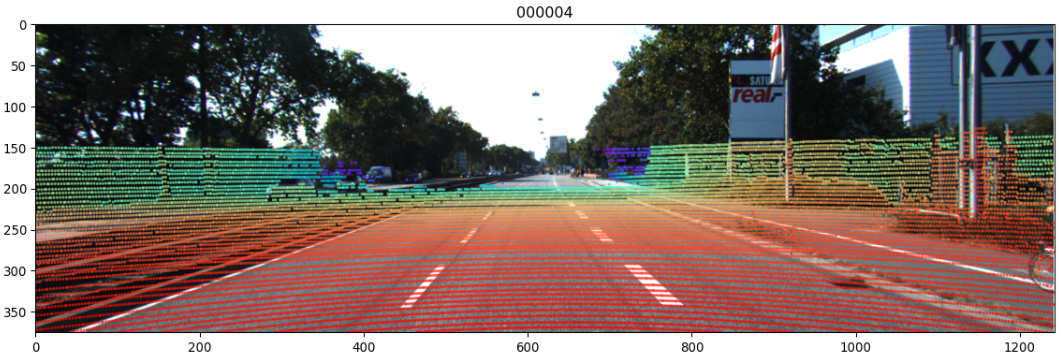
\includegraphics[width=0.8\textwidth]{Book/figures/6_approx_distancia/pcl_projection_kitti2.png}
    \caption{Proyección de la nube de puntos sobre la cámara.}
    \label{fig:Proyección de la nube de puntos sobre la cámara.}
\end{figure}

Mientras que el proceso de segmentación semántica puede ser muy útil y preciso para aproximar la distancia a los objetos del entorno, ya que permite utilizar solo los puntos que se encuentran en los vehículos y no aquellos puntos que no incidan en el objeto de interés, pero se deciden utilizar detecciones 2D ya que con modelos con esta tarea se pueden obtener de manera más rápida dichas detecciones además de diferenciar objetos diferentes si se encuentran muy cerca (cosa que no se puede con un modelo de segmentación semántica). En este análisis por tanto se usará el ground-truth 2D de las imágenes para la realización de las aproximaciones de la distancia a los objetos del entorno.

...

\begin{figure}[H]
    \centering
    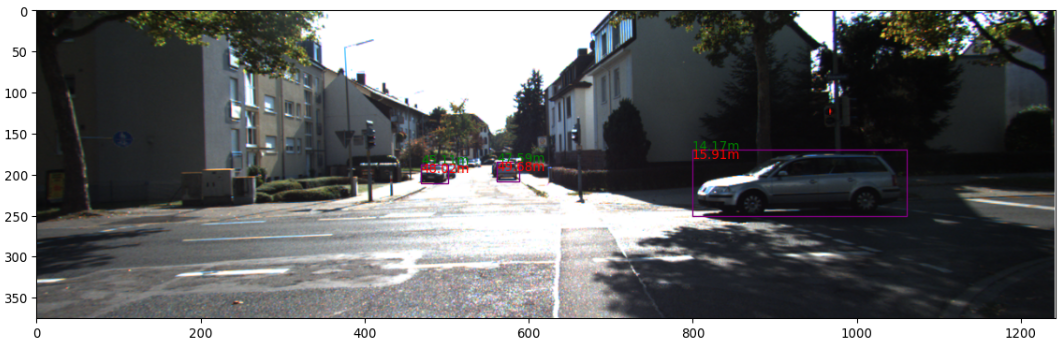
\includegraphics[width=0.8\textwidth]{Book/figures/6_approx_distancia/pcl_projection_distance_kitti2.png}
    \caption{Aproximación de la distancia mediante la nube de puntos.}
    \label{fig:Aproximación de la distancia mediante la nube de puntos.}
\end{figure}

\begin{table}[H]
\centering
\begin{tabular}{|c|c|c|c|c|}
\hline
\textbf{Benchmark (MSE)} & \textbf{Fácil} & \textbf{Moderado} & \textbf{Difícil} & \textbf{Todo}\\ \hline \hline
Coche (distancia)        & 4,084          & 15,759             & 29,198   &42,346         \\ \hline
Peatón (distancia)       & 3,355          & 6,223             & 13,516    &13,500         \\ \hline
Ciclista (distancia)     & 7,134          & 11,968             & 12,902   &12,857        \\ \hline
\end{tabular}
\caption{Evaluación del modelo de aproximación de distancia basado en nube de puntos.}
\label{fig:Evaluación sobre KITTI del primer modelo de aproximación de distancia basado en nube de puntos.}
\end{table}

\begin{figure}[H]
    \centering
    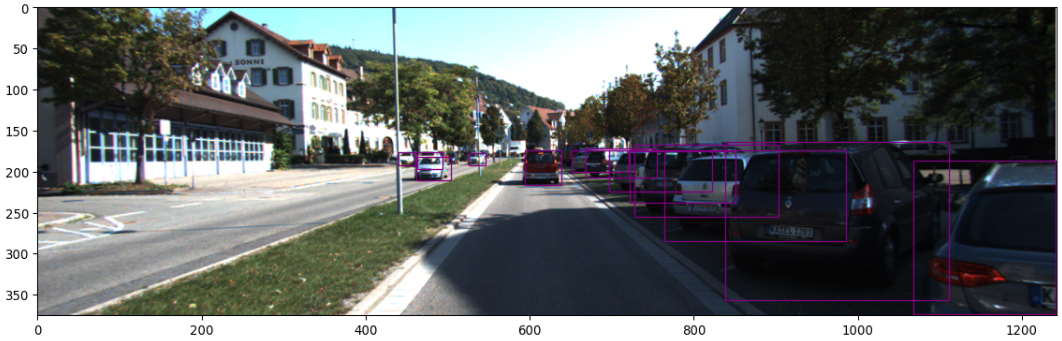
\includegraphics[width=0.8\textwidth]{Book/figures/6_approx_distancia/bb2d_kitti2.png}
    \caption{Caso de dificultad para obtener la distancia a partir de la nube de puntos.}
    \label{fig:Caso de dificultad para obtener la distancia a partir de la nube de puntos.}
\end{figure}

\begin{table}[H]
\centering
\begin{tabular}{|c|c|c|c|c|}
\hline
\textbf{Benchmark (MSE)} & \textbf{Fácil} & \textbf{Moderado} & \textbf{Difícil} & \textbf{Todo}\\ \hline \hline
Coche (distancia)        & 5,143          & 14,861             & 22,961       &29,971     \\ \hline
Peatón (distancia)       & 5,557          & 13,780             & 18,319       &18,032     \\ \hline
Ciclista (distancia)     & 7,107          & 19,733             & 30,106       &25,937  \\ \hline
\end{tabular}
\caption{Evaluación del modelo de aproximación de distancia sin intersecciones en las bounding boxes.}
\label{fig:Evaluación sobre KITTI del primer modelo de aproximación de distancia basado en nube de puntos.}
\end{table}

\subsection{Modelo de rectificación de la distancia}
\label{sec:Modelo de rectificación de la distancia}

\begin{figure}[H]
	\begin{minipage}{0.32\textwidth}
		\centering
		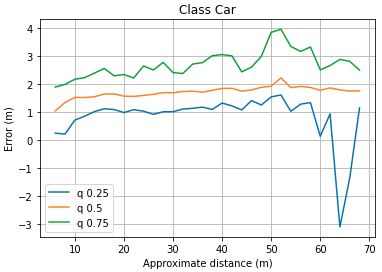
\includegraphics[width=1\linewidth]{Book/figures/6_approx_distancia/error_projection_car_kitti3.png}
	\end{minipage}\hfill
	\begin{minipage}{0.32\textwidth}
		\centering
		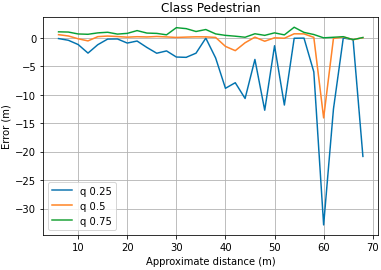
\includegraphics[width=1\linewidth]{Book/figures/6_approx_distancia/error_projection_pedestrian_kitti3.png}
	\end{minipage}\hfill
	\begin{minipage}{0.32\textwidth}
		\centering
		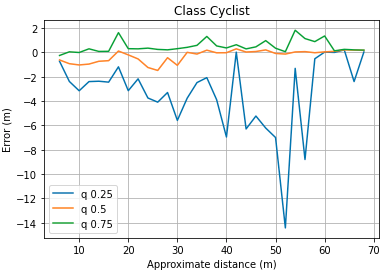
\includegraphics[width=1\linewidth]{Book/figures/6_approx_distancia/error_projection_cyclist_kitti3.png}
	\end{minipage}
	\caption{Error del modelo de de proyección con LiDAR por clase.}
	\label{fig:Error del modelo de de proyección con LiDAR por clase.}
\end{figure}

\begin{figure}[H]
    \centering
    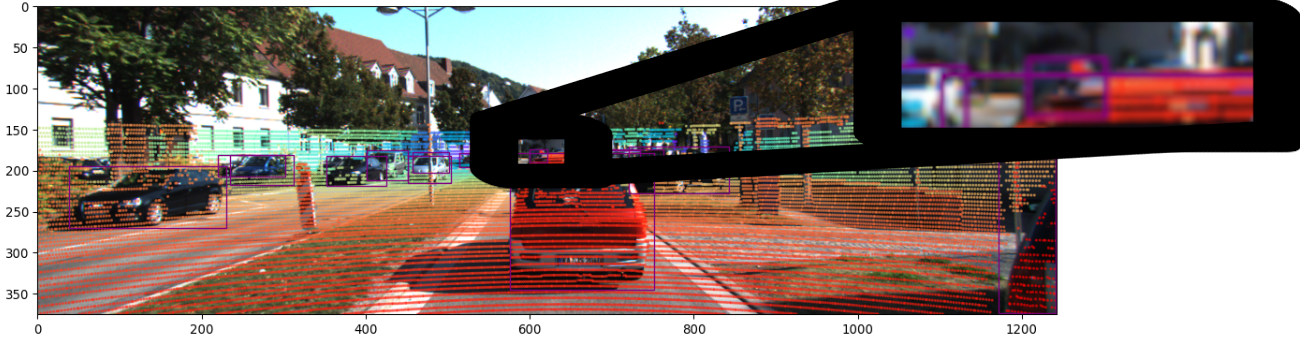
\includegraphics[width=0.8\textwidth]{Book/figures/6_approx_distancia/detail_lidar.png}
    \caption{Caso con gran error en la aproximación de la distancia.}
    \label{fig:Caso con gran error en la aproximación de la distancia.}
\end{figure}

\begin{figure}[H]
	\begin{minipage}{0.32\textwidth}
		\centering
		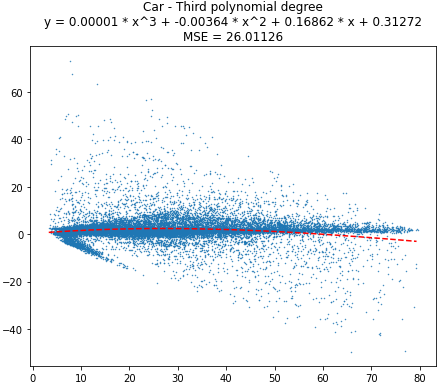
\includegraphics[width=1\linewidth]{Book/figures/6_approx_distancia/rectification_lidar_car.png}
	\end{minipage}\hfill
	\begin{minipage}{0.32\textwidth}
		\centering
		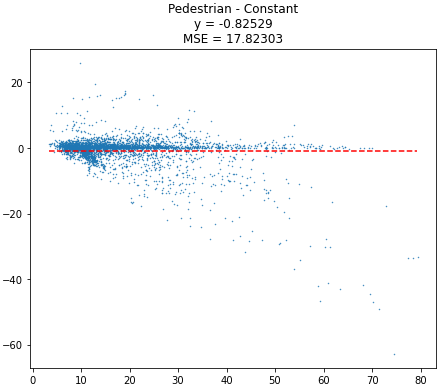
\includegraphics[width=1\linewidth]{Book/figures/6_approx_distancia/rectification_lidar_pedestrian.png}
	\end{minipage}\hfill
	\begin{minipage}{0.32\textwidth}
		\centering
		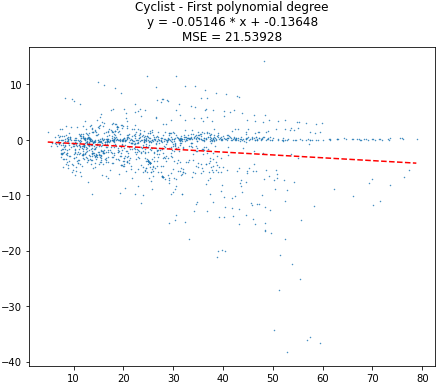
\includegraphics[width=1\linewidth]{Book/figures/6_approx_distancia/rectification_lidar_cyclist.png}
	\end{minipage}
	\caption{Modelo de rectificación de la distancia al centro de los objetos.}
	\label{fig:Modelo de rectificación de la distancia al centro de los objetos.}
\end{figure}

\begin{table}[H]
\centering
\begin{tabular}{|c|c|c|c|c|}
\hline
\textbf{Benchmark (MSE)} & \textbf{Fácil} & \textbf{Moderado} & \textbf{Difícil} & \textbf{Todo}\\ \hline \hline
Coche (distancia)        & 2,201          & 10,309             & 19,310       & 26,011     \\ \hline
Peatón (distancia)       & 5,557          & 13,780             & 18,319       & 18,032     \\ \hline
Ciclista (distancia)     & 4,911          & 15,778             & 24,367       & 21,540  \\ \hline
\end{tabular}
\caption{Evaluación del modelo de aproximación de distancia rectificado.}
\label{fig:Evaluación del modelo de aproximación de distancia rectificado.}
\end{table}

\begin{figure}[H]
	\begin{minipage}{0.32\textwidth}
		\centering
		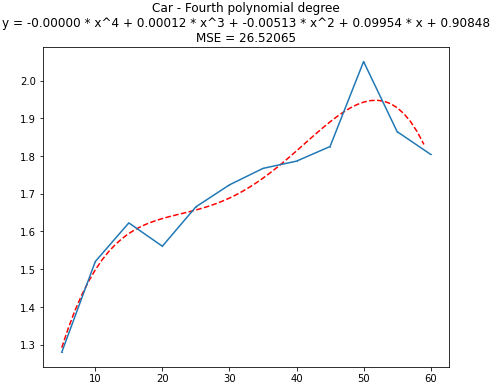
\includegraphics[width=1\linewidth]{Book/figures/6_approx_distancia/rectification2_lidar_car.png}
	\end{minipage}\hfill
	\begin{minipage}{0.32\textwidth}
		\centering
		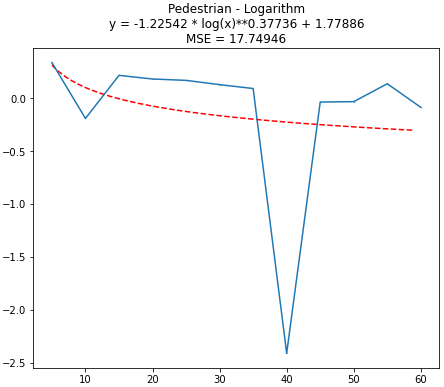
\includegraphics[width=1\linewidth]{Book/figures/6_approx_distancia/rectification2_lidar_pedestrian.png}
	\end{minipage}\hfill
	\begin{minipage}{0.32\textwidth}
		\centering
		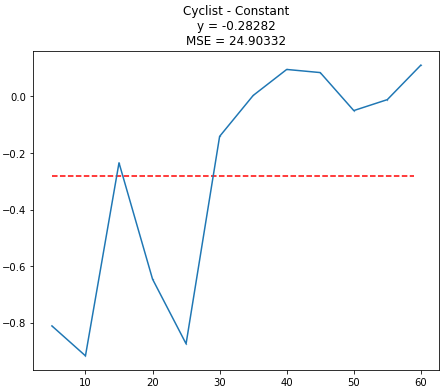
\includegraphics[width=1\linewidth]{Book/figures/6_approx_distancia/rectification2_lidar_cylist.png}
	\end{minipage}
	\caption{Modelo de rectificación de la distancia al centro de los objetos sin outliers.}
	\label{fig:Modelo de rectificación de la distancia al centro de los objetos sin outliers.}
\end{figure}

\begin{table}[H]
\centering
\begin{tabular}{|c|c|c|c|c|}
\hline
\textbf{Benchmark (MSE)} & \textbf{Fácil} & \textbf{Moderado} & \textbf{Difícil} & \textbf{Todo}\\ \hline \hline
Coche (distancia)        & 2,222          & 10,909             & 20,160       & 26,521     \\ \hline
Peatón (distancia)       & 5,467          & 13,691             & 18,198       & 17,912     \\ \hline
Ciclista (distancia)     & 6,404          & 18,799             & 29,000       & 24,903  \\ \hline
\end{tabular}
\caption{Evaluación del modelo de aproximación de distancia rectificado sin outliers.}
\label{fig:Evaluación del modelo de aproximación de distancia rectificado sin outliers.}
\end{table}

\section{Modelo de ensamble}
\label{sec:Modelo de ensamble}

\begin{figure}[H]
    \centering
    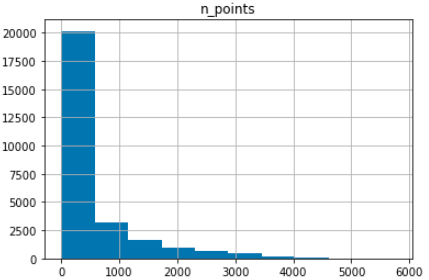
\includegraphics[width=0.4\textwidth]{Book/figures/6_approx_distancia/n_points_hist.png}
    \caption{Histograma con la cantidad de puntos sobre las bounding boxes 2D.}
    \label{fig:Histograma con la cantidad de puntos sobre las bounding boxes 2D.}
\end{figure}

\begin{figure}[H]
	\begin{minipage}{0.32\textwidth}
		\centering
		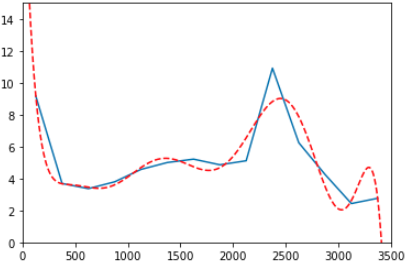
\includegraphics[width=1\linewidth]{Book/figures/6_approx_distancia/ensemble_overfitting_0.png}
	\end{minipage}\hfill
	\begin{minipage}{0.32\textwidth}
		\centering
		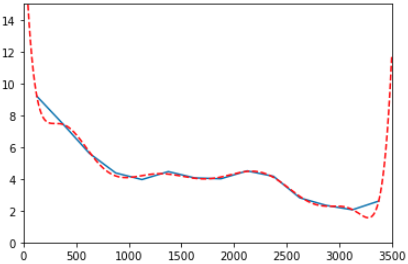
\includegraphics[width=1\linewidth]{Book/figures/6_approx_distancia/ensemble_overfitting_1.png}
	\end{minipage}\hfill
	\begin{minipage}{0.32\textwidth}
		\centering
		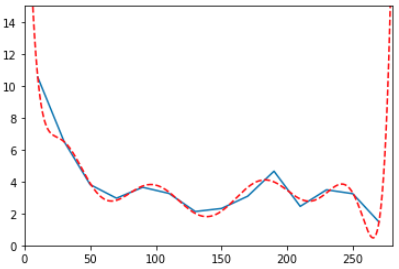
\includegraphics[width=1\linewidth]{Book/figures/6_approx_distancia/ensemble_overfitting_2.png}
	\end{minipage}
	\caption{Ajuste de las funciones de error de los modelos.}
	\label{fig:Ajuste de las funciones de error de los modelos.}
\end{figure}

\begin{figure}[H]
	\begin{minipage}{0.32\textwidth}
		\centering
		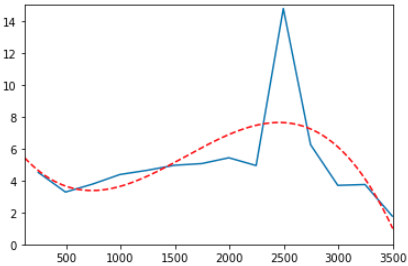
\includegraphics[width=1\linewidth]{Book/figures/6_approx_distancia/ensemble_not_overfitting_0.png}
	\end{minipage}\hfill
	\begin{minipage}{0.32\textwidth}
		\centering
		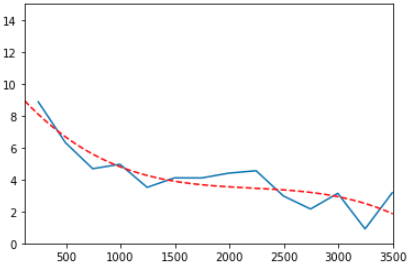
\includegraphics[width=1\linewidth]{Book/figures/6_approx_distancia/ensemble_not_overfitting_1.png}
	\end{minipage}\hfill
	\begin{minipage}{0.32\textwidth}
		\centering
		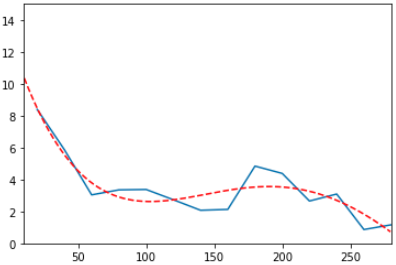
\includegraphics[width=1\linewidth]{Book/figures/6_approx_distancia/ensemble_not_overfitting_2.png}
	\end{minipage}
	\caption{Ajuste de las funciones de error de los modelos sin overfitting.}
	\label{fig:Ajuste de las funciones de error de los modelos sin overfitting.}
\end{figure}

\begin{table}[H]
\centering
\begin{tabular}{|c|c|c|c|}
\hline
\textbf{Benchmark (MSE)} & \textbf{Fácil} & \textbf{Moderado} & \textbf{Difícil}\\ \hline \hline
Coche (distancia)        & 2,137          & 6,499             & 8,618\\ \hline
Peatón (distancia)       & 1,916          & 2,802             & 3,430\\ \hline
Ciclista (distancia)     & 2,214          & 5,038             & 6,335\\ \hline
\end{tabular}
\caption{Evaluación del modelo ensemble utilizando los deciles de los errores.}
\label{fig:Evaluación del modelo ensemble utilizando los deciles de los errores.}
\end{table}

\begin{table}[H]
\centering
\begin{tabular}{|c|c|c|c|}
\hline
\textbf{Benchmark (MSE)} & \textbf{Fácil} & \textbf{Moderado} & \textbf{Difícil}\\ \hline \hline
Coche (distancia)        & 2,061          & 6,824             & 8,863\\ \hline
Peatón (distancia)       & 1,836          & 2,339             & 2,691\\ \hline
Ciclista (distancia)     & 2,007          & 4,26             & 4,834\\ \hline
\end{tabular}
\caption{Evaluación del modelo ensemble utilizando los deciles de los errores cuadráticos.}
\label{fig:Evaluación del modelo ensemble utilizando los deciles de los errores cuadráticos.}
\end{table}

\begin{table}[H]
\centering
\begin{tabular}{|c|c|c|c|}
\hline
\textbf{Benchmark (MSE)} & \textbf{Fácil} & \textbf{Moderado} & \textbf{Difícil}\\ \hline \hline
Coche (distancia)        & 3,011          & 6,608             & 6,972\\ \hline
Peatón (distancia)       & 1,786          & 2,327             & 2,757\\ \hline
Ciclista (distancia)     & 1,542          & 3,030             & 3,379\\ \hline
\end{tabular}
\caption{Evaluación del modelo ensemble utilizando los centiles de los errores.}
\label{fig:Evaluación del modelo ensemble utilizando los centiles de los errores.}
\end{table}

\begin{table}[H]
\centering
\begin{tabular}{|c|c|c|c|}
\hline
\textbf{Benchmark (MSE)} & \textbf{Fácil} & \textbf{Moderado} & \textbf{Difícil}\\ \hline \hline
Coche (distancia)        & 3,721          & 7,459             & 7,286\\ \hline
Peatón (distancia)       & 1,927          & 2,383             & 2,690\\ \hline
Ciclista (distancia)     & 1,540          & 2,611             & 2,631\\ \hline
\end{tabular}
\caption{Evaluación del modelo ensemble utilizando los centiles de los errores cuadráticos.}
\label{fig:Evaluación del modelo ensemble utilizando los centiles de los errores cuadráticos.}
\end{table}

\begin{table}[H]
\centering
\begin{tabular}{|ll|}
\hline
\multicolumn{2}{|c|}{\textbf{Errores}}       \\ \hline
\multicolumn{1}{|l|}{\textbf{1\%}}  & -4.809 \\ \hline
\multicolumn{1}{|l|}{\textbf{5\%}}  & -3.460 \\ \hline
\multicolumn{1}{|l|}{\textbf{50\%}} & -0.372 \\ \hline
\multicolumn{1}{|l|}{\textbf{95\%}} & 4.005  \\ \hline
\multicolumn{1}{|l|}{\textbf{99\%}} & 7.044  \\ \hline
\end{tabular}
\caption{Centiles del error del modelo final de la aproximación de la distancia.}
\label{fig:Centiles del modelo final de la aproximación de la distancia.}
\end{table}

\section{Análisis del error con YOLOv5}
\label{sec:Análisis del error con YOLOv5}

\begin{table}[H]
\centering
\begin{tabular}{|c|c|c|c|}
\hline
\textbf{Benchmark (MSE)} & \textbf{Fácil} & \textbf{Moderado} & \textbf{Difícil}\\ \hline \hline
Coche (distancia)        & 3.296          & 7.349             & 7.072\\ \hline
Peatón (distancia)       & 2.030          & 2.417             & 2.807\\ \hline
Ciclista (distancia)     & 2.207          & 3.787             & 3.803\\ \hline
\end{tabular}
\caption{Evaluación del modelo ensemble sobre las detecciones obtenidas del modelo YOLOv5m.}
\label{fig:Evaluación del modelo ensemble sobre las detecciones obtenidas del modelo YOLOv5m.}
\end{table}